\section{Increasing System Performance}

\begin{concept}{Performance Optimization Trade-offs}\\
\begin{tabular}{|l|l|}
\hline
\textbf{Optimizing for} & \textbf{Drawbacks on} \\
\hline
Higher speed & Power, cost, chip area \\
\hline
Lower cost & Speed, reliability \\
\hline
Zero power consumption & Speed, cost \\
\hline
Super reliable & Chip area, cost, speed \\
\hline
Temperature range & Power, cost, lifetime \\
\hline
\end{tabular}
\end{concept}

\begin{concept}{Instruction Set Architectures}\\
\textbf{RISC (Reduced Instruction Set Computer):}
\begin{itemize}
  \item Few instructions with uniform format
  \item Fast decoding, simple addressing
  \item Less hardware → higher clock rates
  \item More chip space for registers (up to 256)
  \item Load-store architecture reduces memory access
  \item CPU works at full speed on registers
  \item Enables shorter, efficient pipelines 
\end{itemize}

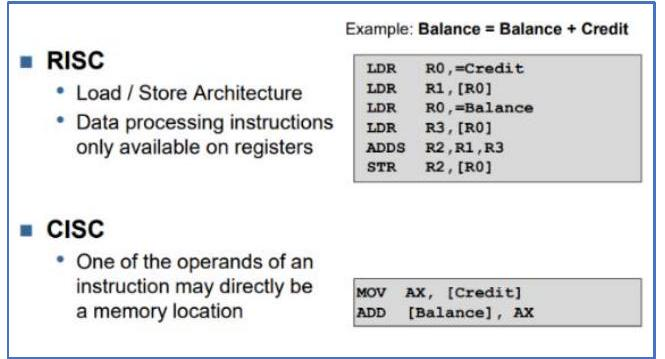
\includegraphics[width=\linewidth]{images/2024_12_29_79e6b22f503fb7b4f718g-13(1)}

\textbf{CISC (Complex Instruction Set Computer):}
\begin{itemize}
  \item More complex instruction set
  \item Lower memory usage for programs
  \item Potential performance gain for short programs
  \item More complex hardware required
\end{itemize}
\end{concept}

\begin{definition}{Computer Architectures}\\
\textbf{Von Neumann Architecture:}
\begin{itemize}
  \item Single memory for program and data
  \item Single bus system between CPU and memory
\end{itemize}

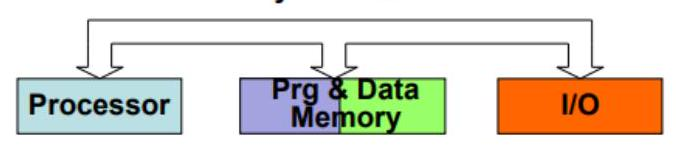
\includegraphics[width=\linewidth]{images/2024_12_29_79e6b22f503fb7b4f718g-13}

\textbf{Harvard Architecture:}
\begin{itemize}
  \item Separate program and data memories
  \item Two sets of address/data buses
  \item Originally from Harvard Mark I
\end{itemize}

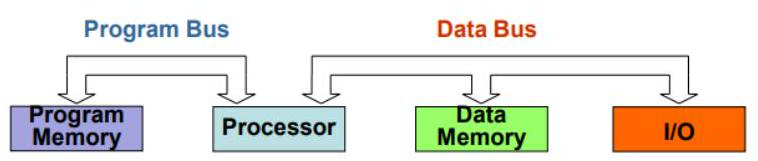
\includegraphics[width=\linewidth]{images/2024_12_29_79e6b22f503fb7b4f718g-13(2)}
\end{definition}

\begin{concept}{Pipelining}\\
Process of fetching next instruction while current one decodes:

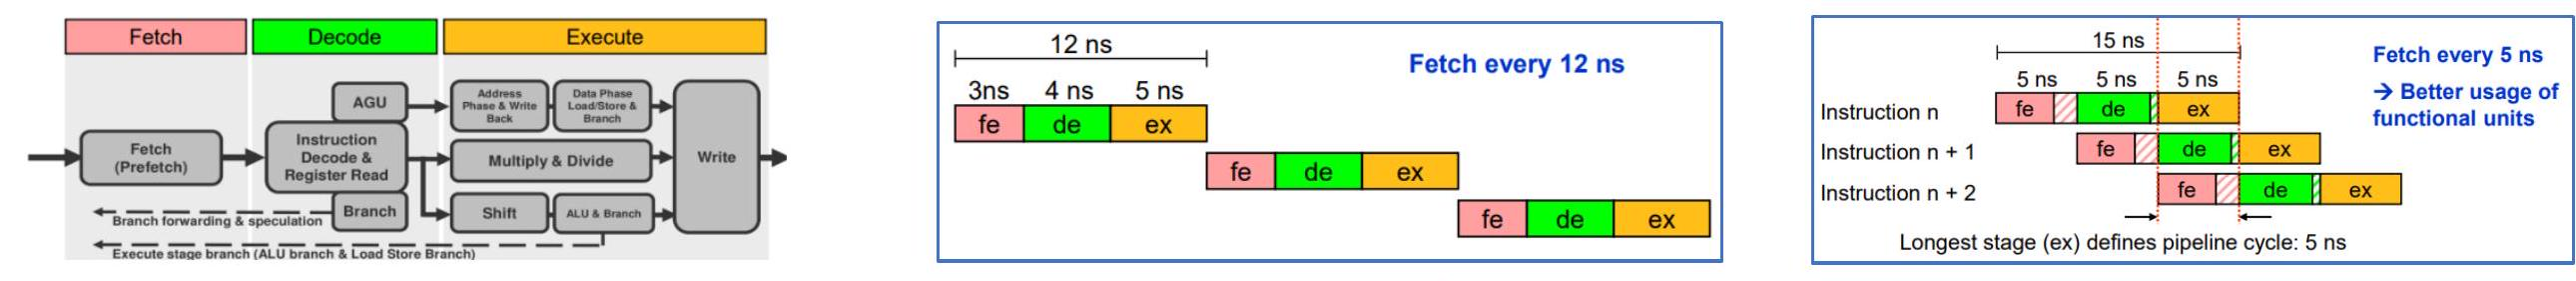
\includegraphics[width=\linewidth]{images/2024_12_29_79e6b22f503fb7b4f718g-14(2)}

\textbf{Pipeline Stages (Example):}
\begin{itemize}
  \item Fetch (Fe): Read instruction - 3ns
  \item Decode (De): Process instruction - 4ns
  \item Execute (Ex): Execute and writeback - 5ns
\end{itemize}

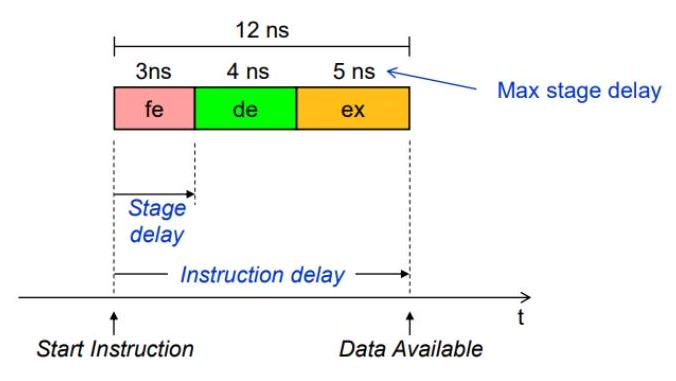
\includegraphics[width=\linewidth]{images/2024_12_29_79e6b22f503fb7b4f718g-14(1)}

\textbf{Advantages:}
\begin{itemize}
  \item Uniform execution time per stage
  \item Significant performance improvement
  \item Simpler hardware per stage
\end{itemize}

\textbf{Disadvantages:}
\begin{itemize}
  \item Blocking stages affect whole pipeline
  \item Memory access conflicts between stages
\end{itemize}
\end{concept}

\begin{definition}{Pipeline Performance}\\
Without pipelining:
\[\frac{\text{Instructions}}{\text{second}} = \frac{1}{\text{Instruction delay}}\]

With pipelining:
\[\frac{\text{Instructions}}{\text{second}} = \frac{1}{\text{Max stage delay}}\]

Note: Pipeline must be filled first
\end{definition}

\begin{example2}{Pipeline Execution}\\
\textbf{Optimal Case:}
\begin{itemize}
  \item Register-only operations
  \item 6 instructions in 6 cycles
  \item CPI = 1 (Cycles Per Instruction)
\end{itemize}

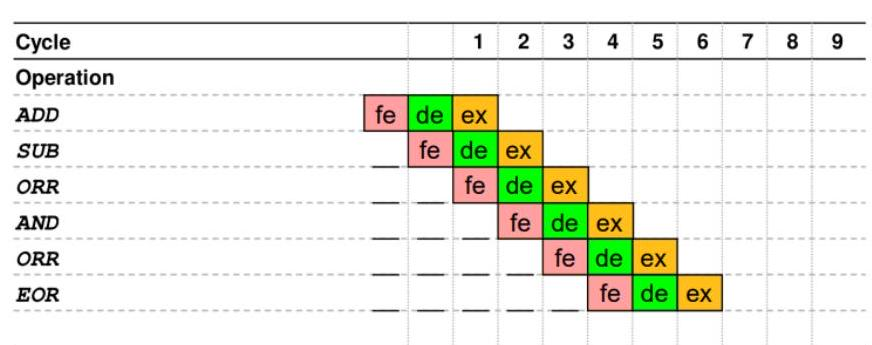
\includegraphics[width=\linewidth]{images/2024_12_29_79e6b22f503fb7b4f718g-14}

\textbf{LDR Special Case:}
\begin{itemize}
  \item 6 instructions in 7 cycles due to memory access
  \item Pipeline stalls for memory read
  \item CPI = 1.2
\end{itemize}
\end{example2}

\begin{concept}{Pipeline Hazards and Optimization}\\
\textbf{Control Hazards:}
\begin{itemize}
  \item Branch decisions in execute stage
  \item Pipeline stalls for taken branches
\end{itemize}

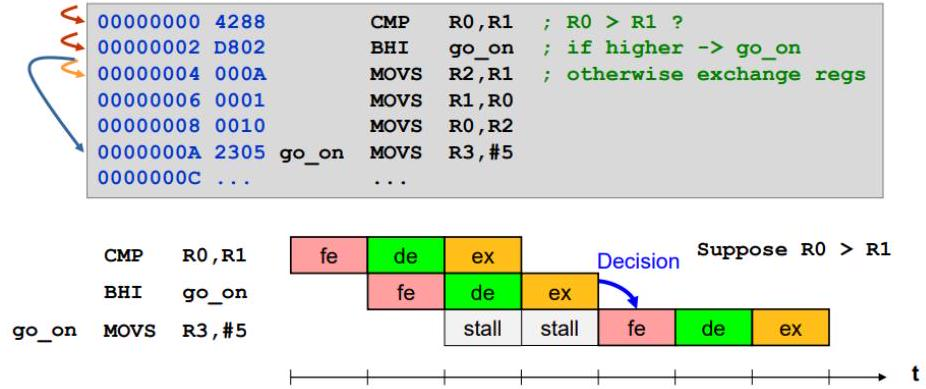
\includegraphics[width=\linewidth]{images/2024_12_29_79e6b22f503fb7b4f718g-15}

\textbf{Optimization Techniques:}
\begin{itemize}
  \item Branch prediction based on history
  \item Instruction prefetch
  \item Out-of-order execution
\end{itemize}

\textbf{Optimization Limits:}
\begin{itemize}
  \item Security vulnerabilities (Meltdown, Spectre)
  \item Complex optimizations increase risk
\end{itemize}
\end{concept}

\begin{concept}{Parallel Computing}\\
Different approaches to parallelism:
\begin{itemize}
  \item \textbf{Vector Processing}: Single instruction processes multiple data
  \item \textbf{Multithreading}: Multiple threads share CPU
  \item \textbf{Multicore}: Multiple CPU cores on one chip
  \item \textbf{Multiprocessor}: Multiple CPUs in system
\end{itemize}
\end{concept}

\begin{KR}{Optimizing System Performance}\\
Steps for performance optimization:
\begin{enumerate}
  \item Analyze performance bottlenecks
  \item Choose appropriate architecture:
    \begin{itemize}
      \item RISC vs CISC based on application
      \item Consider memory architecture
    \end{itemize}
  \item Implement pipelining:
    \begin{itemize}
      \item Balance stage delays
      \item Handle hazards appropriately
    \end{itemize}
  \item Consider parallelization options
  \item Evaluate security implications
\end{enumerate}
\end{KR}

\begin{concept}{Performance Growth Overview}\\
Historical development:
\begin{itemize}
  \item Early improvements:
    \begin{itemize}
      \item Increasing clock frequencies
      \item Better manufacturing processes
      \item Smaller transistor sizes
    \end{itemize}
  \item Modern improvements:
    \begin{itemize}
      \item Advanced architectural concepts (RISC, Pipelining)
      \item Multiple cores
      \item Specialized hardware units
    \end{itemize}
  \item Current limitations:
    \begin{itemize}
      \item Power density
      \item Heat dissipation
      \item Memory wall
      \item Parallelization overhead
    \end{itemize}
\end{itemize}
\end{concept}

\begin{concept}{System Level Optimization}\\
Different approaches to improve performance:
\begin{itemize}
  \item \textbf{External Factors}:
    \begin{itemize}
      \item Better compiler optimization
      \item Improved algorithms
      \item Efficient software design
    \end{itemize}
  \item \textbf{System Level Factors}:
    \begin{itemize}
      \item Special Purpose Units (e.g., Crypto, Video)
      \item Multiple Processors
      \item Bus Architecture optimization
      \item Faster peripheral components
    \end{itemize}
  \item \textbf{CPU Improvements}:
    \begin{itemize}
      \item Increased Clock Speed
      \item Cache Memory
      \item Multiple Cores
      \item Pipeline Optimization
      \item Branch Prediction
      \item Out-of-Order Execution
    \end{itemize}
\end{itemize}
\end{concept}

\begin{formula}{Pipeline Performance Calculation}\\
For a processor with n pipeline stages:

\textbf{Without pipelining:}
\begin{itemize}
  \item Time per instruction = Sum of all stage delays
  \item Performance = $\frac{1}{\text{Total delay}}$
\end{itemize}

\textbf{With pipelining:}
\begin{itemize}
  \item Time per instruction = Longest stage delay
  \item Initial latency = n cycles
  \item Throughput = $\frac{1}{\text{Max stage delay}}$
\end{itemize}

Example calculation:
\begin{itemize}
  \item Stage delays: Fe=3ns, De=4ns, Ex=5ns
  \item Without pipeline: 12ns per instruction
  \item With pipeline: 5ns per instruction after filling
  \item Performance improvement: 2.4×
\end{itemize}
\end{formula}

\begin{example2}{Pipeline Hazards}
Three types of pipeline hazards:

1. \textbf{Structural Hazards}:
\begin{lstlisting}[style=basesmol]
LDR  R0, [R1]    ; Needs memory access
LDR  R2, [R3]    ; Also needs memory access
; Memory system can't handle both at once
\end{lstlisting}

2. \textbf{Data Hazards}:
\begin{lstlisting}[style=basesmol]
ADDS R0, R1, R2  ; R0 gets new value
ADDS R3, R0, R4  ; Uses R0 before ready
; Second instruction must wait
\end{lstlisting}

3. \textbf{Control Hazards}:
\begin{lstlisting}[style=basesmol]
CMP  R0, #0      ; Compare
BEQ  target      ; Branch if equal
ADD  R1, R2, R3  ; May be unnecessary
SUB  R4, R5, R6  ; May be unnecessary
target
; Pipeline must flush if branch taken
\end{lstlisting}
\end{example2}

\begin{concept}{Parallel Processing Models}\\
\textbf{SISD (Single Instruction Single Data):}
\begin{itemize}
  \item Traditional sequential processing
  \item One instruction processes one data item
  \item Example: Basic scalar processor
\end{itemize}

\textbf{SIMD (Single Instruction Multiple Data):}
\begin{itemize}
  \item Vector processing
  \item One instruction processes multiple data items
  \item Examples: MMX, SSE, AVX instructions
\end{itemize}

\textbf{MIMD (Multiple Instruction Multiple Data):}
\begin{itemize}
  \item True parallel processing
  \item Multiple processors execute different instructions
  \item Example: Multicore systems
\end{itemize}
\end{concept}

\begin{KR}{Performance Optimization Guidelines}\\
Steps for system optimization:

1. \textbf{Analyze Requirements}:
\begin{itemize}
  \item Performance targets
  \item Power constraints
  \item Cost limitations
  \item Reliability needs
\end{itemize}

2. \textbf{Choose Architecture}:
\begin{itemize}
  \item RISC vs CISC
  \item Memory architecture
  \item Pipeline depth
  \item Parallelization approach
\end{itemize}

3. \textbf{Optimize Implementation}:
\begin{itemize}
  \item Balance pipeline stages
  \item Implement hazard handling
  \item Consider branch prediction
  \item Optimize memory access
\end{itemize}

4. \textbf{Security Considerations}:
\begin{itemize}
  \item Evaluate optimization risks
  \item Consider side-channel attacks
  \item Balance performance and security
\end{itemize}
\end{KR}

\begin{example2}{Multicore vs Multiprocessor}
Key differences:
\begin{itemize}
  \item \textbf{Multicore}:
    \begin{itemize}
      \item Multiple CPU cores on single chip
      \item Shared cache and memory interface
      \item Lower communication overhead
      \item More power efficient
    \end{itemize}
  \item \textbf{Multiprocessor}:
    \begin{itemize}
      \item Multiple separate CPU chips
      \item Independent caches
      \item Higher communication overhead
      \item More scalable for large systems
    \end{itemize}
\end{itemize}
\end{example2}

